\documentclass{article}
\usepackage[utf8]{inputenc}
\usepackage[T1]{fontenc}
\usepackage{graphicx}
\usepackage{amsmath}
\usepackage{wrapfig}
\usepackage[top=1in, bottom=1.25in, left=1.1in, right=1.1in]{geometry}

\title{Reporte - Actividad 2}
\author{García Monge Itzel Alexia}
\date{7 de Febrero, 2018}

\begin{document}
\maketitle

\section{Introducción}
Durante la realización de esta actividad se logró aprender algunos usos básicos de Pyhton, como lo es correr una celda, descargar y leer documentos, hacer gráficas, crear tablas, y obtener los valores máximos y mínmos. Todo esto mediante el kernel que es Jupyter Notebook, el cual se abre y cierra desde la terminal de una computadora, y corre en línea.

\section{Resumen}
Para poder utilizar Jupyter Notebook se selecciona una carpeta en $Archivos$ y se abre un terminal donde se escribe $Jupyter Notebook$, lo cual abrirá la página de inicio de Jupyter en Google Chrome. Se selecciona en $New$ la opción de Pyhton3.0, nombramos la pestaña como $Actividad2$ y estamos listos para programar Pyhton en línea.
	
	Para esta actividad se visitó la página del Servicio Meteorológico Nacional y se seleccionaron los datos de la ciudad Rio Tomatlan, localizado en el estado de Guadalajara. Se guardaron los datos de los vientos con un periodo de 60 minutos en la carpeta de $Actividad2$,siendo estos los datos que se trabajarán.
    
\subsection{Pandas, Numpy y Matplotlib}
Antes de poder iniciar a programar, se tiene que cargar a la memoria de nuestras celdas tres bibliotecas muy importantes: pandas, matplotlib.pyplot y numpy. Pandas es una bilbioteca de software específicamente para la programación en Python usada en el manejo de manipulación de datos y análisis. Numpy es un paquete indispensable si se desea hacer física computacional en Python, ofreciendo la habilidad de utilizar matrices n-dimensionales, transformaciones de Fourier, e incluso poder integrar códigos externos como C, C++ y Fortran. Por su parte, matplotlib.pyplot es una biblioteca de trazado para Python en 2 dimensiones, facilitando la creación de gráficas. 
    
    Al cargarlas a las celdas, se recomienda abreviar sus nombres para facilitar su uso al programar. La manera de cargarlas a las celdas de trabajo es escribiendo:
   
    \begin{verbatim}import pandas as pd
	import numpy as np
	import matplotlib.pyplot as plt
    \end{verbatim}
    
    Se corre la celda con la combinación de teclas $"Shift + Enter"$. Esto, además de correr la celda programada, también crea inmediatamente una nueva celda limpia para seguir programando algo nuevo abajo de la otra.
    
\subsection{Uso Básico de los Comandos}
\subsubsection{Leer un Documento}
Cuando se tiene un docuemnto con el cual deseas trabajar, el primer paso que debes realizar es poder leer sus datos; lo cual es posible con pandas. Para hacerlo, debemos nombrar una variable que guarde la información del documento seguido de un igual y procedemos a escribir el comando $pd.read_csv()$. $pd$ siendo pandas, y $read_cvs()$ siendo la función para leer el documento. Dentro del paréntesis se ecribe entre apóstrofes el nombre del documento con su extensión. 

	Pero ya que en Pyhton lo único que se quiere leer son sus datos, y por lo general los documentos empiezan con títulos y explicaciones acerca de su contenido, se agrega la función $skiprows=$ para no leer el docuemnto hasta desopués de cierto número de líneas.
    
    Digamos que queremos leer todo el documento de $Rio$ $Tomatlan$, este se programaría de la siguiente forma:
     \begin{verbatim}
    df0 = pd.read_csv('RioTomatlan.TXT', skiprows=4, sep='\s+')
    \end{verbatim}

    El leer el documento no significa que este se imprimirá en pantalla al momento de correr la celda. Si se desea imprimir líneas del documento que se ha guardado se utiliza la función $head()$, agregando en paréntesis la cantidad de líneas. Si no se le agrega ningúna cantidad en los paréntesis, se imprimen por default las primeras 5 línes. 
    
    Digamos querer saber los primeros 10 renglones de $Rio$ $Tomatlan$, programamos $df0.head(10)$ y obtenemos:
    
    \begin{center}
    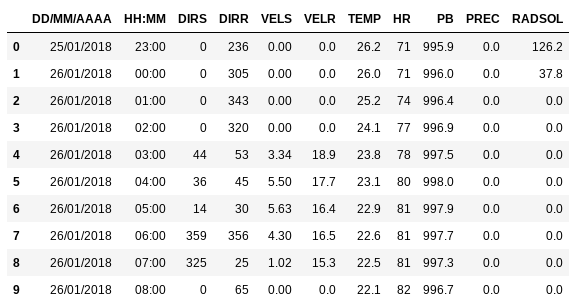
\includegraphics[height=6cm]{head.png}
	\end{center}
    
\subsubsection{Estructura y Tipo de Datos}
Pyhton no puede leer los textos y asumir que están en una columna, primero se deben leer y acomodar. Con Pandas, usando la función $DataFrame()$, creamos una variable que vaya a contener los datos con la estructura, un igual, y la función $pd.DaraFrame()$. Por ejemplo
    
    \begin{verbatim}df = pd.DataFrame(df0) \end{verbatim} sería para darle estructura a la variable $df0$.
    
    Si queremos saber qué tipo de datos está leyendo Pandas, utilizamos la función $df.dtypes$. Al correr la celda, una tabla como la siguiente aparecerá:
    
    \begin{center}
    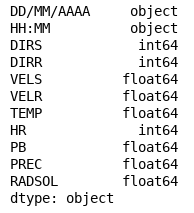
\includegraphics[height=5cm]{types.png}
    \end{center}
    
\subsubsection{Mezclar Columnas}
    Para mezclar la información de columnas y crear una nueva con los datos, se selecciona la variable cdeseada y agregamos en corchetes el nombre de la nueva columna seguido de un igual, seguido de la función $pd.to_datetime()$. Dentro del paréntesis utilizamos Pandas de nuevo para especificar cuáles columnas queremos con $df.apply()$. Dentro de ese paréntesis escribimos los nombres de las columnas a mezclar utilizando la función anónima $lambda$. Las funciones anónimas son aquellas que no necesitan declararse como el resto de las demás funciones. 
    
    Regresando con nuestro ejemplo de $Rio$ $Tomatlan$, al mezclar la columna del día y la hora:
    
    %Para escribir exactamente lo que queremos sin identificarlo como lenguaje de Latex
    \begin{verbatim}
    df['FECHA'] = pd.to_datetime(df.apply(lambda x: x['DD/MM/AAAA'] + ' ' + x['HH:MM'], 
    1), dayfirst=True)
    \end{verbatim}
    
	Donde las sumas expresan qué más se desea mezclar con la columna mencionada, recordemos que entre las columnas hay un espcacio en blanco, es por eso que se agregan las apóstrofes con el especio.
    
\subsubsection{Eliminar Columnas}
    Para eliminar columnas escrbimos la variable que contiene las columnas a eliminar, escribimos el nombre de la variable una vez más, seguido de un punto y la palabra $drop()$. Dentro de los paréntesis nombramos entre apóstrofes las columnas a eliminar.
    
    Si queremos eliminar las columnas con el día y la hora, pues ya no son necesarias. escribimos:
    
    \begin{verbatim}
    df = df.drop(['DD/MM/AAAA', 'HH:MM'], 1)
    \end{verbatim}

\subsubsection{Análisis Exploratorio de Datos}
Cuando se tienen una gran cantidad de datos es difícil tener una idea general de ellos. El análisis exploratorio de datos en Pyhton te ofrece una tabla donde con la cantidad de datos, la media, estándar, mínima, primer, segundo y tercer cuartil, y el valor máximo de cada columna. Se obtiene escribiendo el nombre de tu variable seguido de un punto y el comando $describe()$.
    
    El análisis exploratorio de datos de $Rio$ $Tomatlan$ es
    
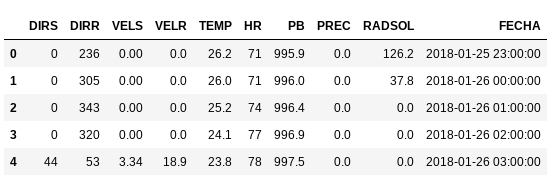
\includegraphics[height=5cm]{Analisis_de_datos.png}

\subsubsection{Mostrar ciertos Datos en Tablas}
Casi siempre en la realización de experimentos físicos, los valores que nos interesan están entre cierto rango numérico. Volvamos al ejemplo de $Rio$ $Tomatlan$ y supongamos que queremos saber los valores sólo cuando su temperatura varia entre los 24 y 25 $^\circ$C. 
    
    Se crea variable que contenga los datos en donde la columna de $TEMP$ tenga valores mayores a 24$^\circ$C. Luego se hace otra variable donde se busca que los datos de $TEMP$ en la nueva variable sean menores de 25. Esto hace que la nueva variable tenga todos los datos del archivo cuando la temperatura era mayor que 24 pero menor que 25. Se programa como:
    
    \begin{verbatim}df_tmp = df[df.TEMP > 24] 
	df_select = df_tmp[df_tmp.TEMP < 25]
	df_select
    \end{verbatim}
    y se obtiene la tabla:
    
    \begin{center}
    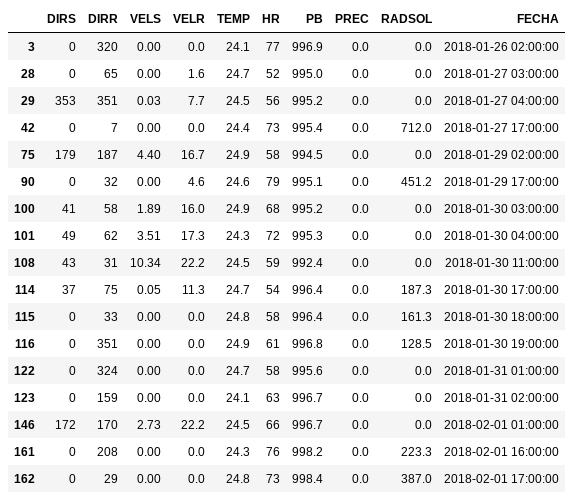
\includegraphics[height=10cm]{Temp_24_25.png}
    \end{center}
    
\subsubsection{Promedios}
Si se necesita saber el valor promedio de todos los datos, se escribe $variable.mean()$. Al correr la celda obtienes una tabla con los valores promedios de todas las columnas. Cuando se desea saber el promedio de una sóla columna se escribe $variable.Nom_Columna.mean()$ y se imprime el valor.
   
   \begin{center}
   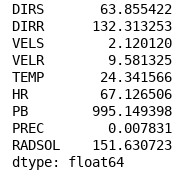
\includegraphics[height=5cm]{promedios.png}{Promedios Rio Tomatlan} 
   \end{center}
   
\subsection{Gráficas}
Teniendo el paquete de matplotlib, podemos crear varios tipos de gráficas. Digamos que queremos programar la rapidez de los vientos de $Rio$ $Tomatlan$, y programamos:

\begin{verbatim}plt.figure(); df.VELS.plot(); plt.legend(loc='best')
plt.title("Variación de la Rapidez de los Vientos")
plt.ylabel("Rapidez (m/s)")
plt.grid(True)
plt.show()
\end{verbatim}

	$Figure$ nos indica que quiere hacer una gráfica, mientras que $df.VELS.plot$ dice qué desea graficar. $plt.legend(loc='best')$ hara que las leyendas se asignen en donde mejor se acomoden. $Title$, $ylabel$ y $xlabel$ nos permite darle título a la gráfica y sus ejes, mientras que $grid$ muestra la cuadrícula. La gráfica se creará pero no se imprimirá a menos que se escriba la función $plt.show()$.
    
    Al final obtenemos la gráfica:
    
   \begin{center}
   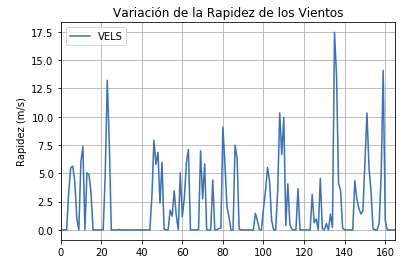
\includegraphics[height=6cm]{grafica_de_los_vientos.png}
   \end{center}

	Hay veces que queremos tener dos valores en la misma gráfica, para lo que se escribe
    
    \begin{verbatim}
    df1 = df[['TEMP','HR']]
    \end{verbatim}
    
    antes del resto del código. $Df1$ siendo una nueva variable, $TEMP$ y $HR$ son las columnas que se van a graficar de la variable $df$, obteniendo:

	\begin{center}
    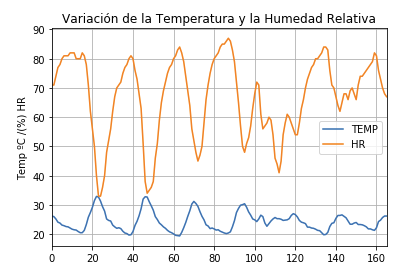
\includegraphics[height=6cm]{con_dos.png}
    \end{center}
    
    En lugar de programar el primer renglón del principio, podemos hacer una gráfica en función de otra escribiendo qué va en cada eje con 
    
    \begin{verbatim}
    plt.plot_date(x=df.FECHA, y=df.TEMP, fmt="b-")
    \end{verbatim}
    
    Siendo $plot_date()$ la función para asignar los ejes. $Fmt$ es el formato, podemos asignarle color con la primera letra de cada color en inglés, y decidir si la gráfica es de puntos o se conectan con líneas dejando vacío o escribiendo $"-"$.
    
    \begin{center}
    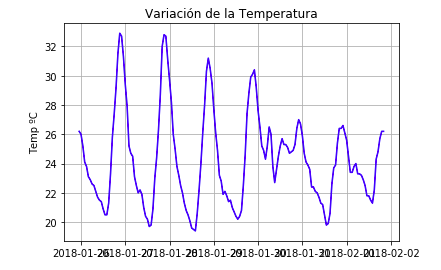
\includegraphics[height=6cm]{ejesxy.png}
    \end{center}
    

    Entonces, si deseamos tener una gráfica con dos datos, pero queremos asignarle una cloumna a cada eje, simplemente escribimos dos veces la línea de programación anterior y obtenemos:
    
    \begin{center}
    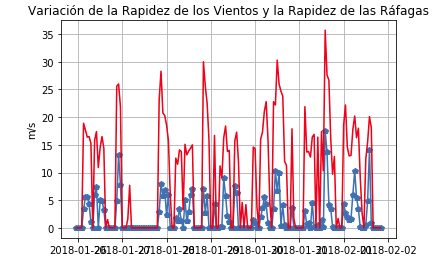
\includegraphics[height=6cm]{dosconejes.png}
    \end{center}
    
	Algunos otros ejemplos de los tipos de gráficas que podemos obtener son:
    
    \begin{center}
    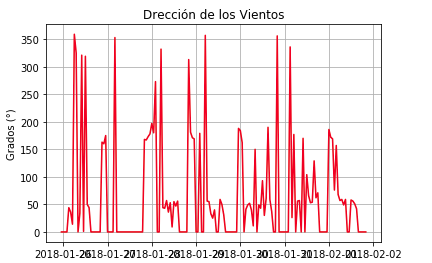
\includegraphics[height=6cm]{dirvientos.png}
    \end{center}
    
    \begin{center}
    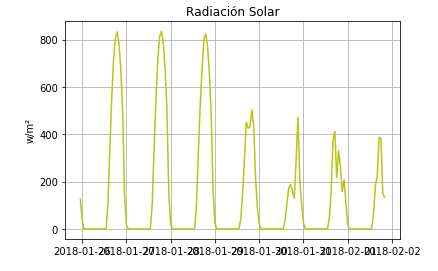
\includegraphics[height=6cm]{RADSOLAR.png}
    \end{center}
    
    Podemos ver que la radiación en función del tiempo presenta picos durante ciertos momemtos del día para bajar rapidamente al caer la noche, teniendo la ciudad una diferencia de temperatura de $13.5$ $\circ$C. Esta gráfica hace relación con la Gráfica de Humedad Relativa, ya que entre menos radiación solar hay, menor la temperatura, que en consecuencia trae menos humedad.

\section{Apéndice}
\begin{enumerate}
\item \textbf{¿Cuál es tu primera impresión de Jupyter Notebook?}
Me pareció difícil de creer podíamos programar en línea de manera tan sencilla y eficiente, pues las otras veces que usé algún compilador en línea la lentitud pobre manejo de las funciones era muy frustrante. Además, fue sorprendente ver que el acceso es en base a la terminar de nuestra computadora.

\item \textbf{¿Se te dificultó leer código en Python?}
Al principio, al no tener ninguna introducción al lenguaje de programación, no logré identificar la mayoría de las funciones y variables, pero al momento de realizar el reporte, fui encontrando sentido al manejo de estás y descubrí que son relativamente fáciles de comprender, y aún más fáciles de usar.

\item \textbf{¿En base a tu experiencia de programación en Fortran, que te parece el entorno de trabajar en Python?}
Es muy distinto, en general me pone algo incómoda el no declarar todas las variables que usaremos desde un principio, además de tener la libertad de correr funciones por separado, un pedazo de programa siendo independiente del otro. 

\item \textbf{A diferencia de Fortran, ahora se producen las gráficas utilizando la biblioteca Matplotlib. ¿Cómo fue tu experiencia?}
Fue lo que más me tomó tiempo comprender, pero una vez que comprendes lo que hace cada cosa, es fácil encontrar su lógica, así como crear nuevas gráficas. Sin mencionar que es mucho más cómo poder crear las gráficas en las mismas celdas donde se programa lo demás y que se impriman ahí mismo.

\item \textbf{En general, ¿qué te pereció el entorno de trabajo en Python?}
Cómodo, me fascinó la idea de poder programas "pedazos" y correrlos, así, al momento de tener un error, reduzco el mis dificuultades de encontrarlos, además los resolvería mucho más ráido.

\item \textbf{¿Qué opinas de la actividad? ¿Estuvo compleja? ¿Mucho material nuevo? ¿Que le faltó o que le sobró?}
La actividad en sí fue sencilla, pero era demasiado material nuevo sin tener ningun tipo de introducción hacia lo que era. Los ejemplos proporcionados no daban mucha información de qué era cada cosa, no podía diferenciar lo que era una función y lo que era una variable. Lo que le dió toda la dificultad a la actividad fue el hecho de ser material nuevo presentado sin ninguna preparación para el alumno.

\item \textbf{¿Qué modificarías para mejorar?}
Primero dedicaría una o dos clases para la explicación basica del código de Python, por ejemplo, el hecho de que aquí no es necesario declarar las variables no nos prepara para diferenciar variables que pueden ser creadas y funciones que ayudan al programa. Aún no comprendo qué hace cada comando, si tuviera que programar algo, no sería capaz de recordar que hace cada cosa porque no lo entiendo del todo.

\item \textbf{¿Comentarios adicionales que desees compartir?}
Me gustaría tener una idea más clara de lo que voy a hacer al momento de iniciar una actividad, el hecho de llegar y empezar a realizar ejemplos causa que tarde más en comprender qué es lo que hace cada cosa y qué es lo que es sólo texto.

\section{Bibliografía}
\begin{itemize}
\item Pyplot tutorial. Retrieved February 03, 2018

$https://matplotlib.org/users/pyplot_tutorial.html$

\item NumPy. Retrieved February 03, 2018

$http://www.numpy.org/$

\item Introduction. Retrieved February 03, 2018

$https://matplotlib.org/$

\item Ordenamiento y máximos y mínimos de un arreglo con Python. (2013, December 21). Retrieved February 03, 2018

$https://joseguerreroa.wordpress.com/2013/12/09/ordenamiento-y-maximos-y-minimos-de-un-arreglo-con-python/$

\item Using Pandas for Analyzing Data - Data Munging. Retrieved February 03, 2018

$http://wavedatalab.github.io/datawithpython/munge.html$
\end{itemize}
\end{enumerate}

\end{document}
